%%%%%%%%%%%%%%%%%%%%%%%%%%%%%%%%%%%%%%%%%
% Beamer Presentation
% LaTeX Template
% Version 1.0 (10/11/12) 
%
% This template has been downloaded from:
% http://www.LaTeXTemplates.com
%
% License:
% CC BY-NC-SA 3.0 (http://creativecommons.org/licenses/by-nc-sa/3.0/)
%
%%%%%%%%%%%%%%%%%%%%%%%%%%%%%%%%%%%%%%%%%

%----------------------------------------------------------------------------------------
%	PACKAGES AND THEMES
%----------------------------------------------------------------------------------------

\documentclass{beamer}

\mode<presentation> {
%\mode<handouts> {
%\mode<article> {


% The Beamer class comes with a number of default slide themes
% which change the colors and layouts of slides. Below this is a list
% of all the themes, uncomment each in turn to see what they look like.


%\usetheme{default}
%\usetheme{AnnArbor}
%\usetheme{Antibes}
%\usetheme{Bergen}
%\usetheme{Berkeley}
%\usetheme{Berlin}
%\usetheme{Boadilla}
\usetheme{CambridgeUS}
%\usetheme{Copenhagen}
%\usetheme{Darmstadt}
%\usetheme{Dresden}
%\usetheme{Frankfurt}
%\usetheme{Goettingen}
%\usetheme{Hannover}
%\usetheme{Ilmenau}
%\usetheme{JuanLesPins}
%\usetheme{Luebeck}
%\usetheme{Madrid}
%\usetheme{Malmoe}
%\usetheme{Marburg}
%\usetheme{Montpellier}
%\usetheme{PaloAlto}
%\usetheme{Pittsburgh}
%\usetheme{Rochester}
%\usetheme{Singapore}
%\usetheme{Szeged}
%\usetheme{Warsaw}

% As well as themes, the Beamer class has a number of color themes
% for any slide theme. Uncomment each of these in turn to see how it
% changes the colors of your current slide theme.

%\usecolortheme{albatross}
\usecolortheme{beaver}
%\usecolortheme{beetle}
%\usecolortheme{crane}
%\usecolortheme{dolphin}
%\usecolortheme{dove}
%\usecolortheme{fly}
%\usecolortheme{lily}
%\usecolortheme{orchid}
%\usecolortheme{rose}
%\usecolortheme{seagull}
%\usecolortheme{seahorse}
%\usecolortheme{whale}
%\usecolortheme{wolverine}

%\setbeamertemplate{footline} % To remove the footer line in all slides uncomment this line
%\setbeamertemplate{footline}[page number] % To replace the footer line in all slides with a simple slide count uncomment this line

%\setbeamertemplate{navigation symbols}{} % To remove the navigation symbols from the bottom of all slides uncomment this line
}

\usepackage{graphicx} % Allows including images
\graphicspath{{../figures}}
\usepackage{booktabs} % Allows the use of \toprule, \midrule and \bottomrule in tables
\usepackage{amsmath, amssymb, amsthm, gensymb,mathrsfs}%,eufrak}
\usepackage{hyperref}
\usepackage{tabularx}
\usepackage{longtable}
\usepackage{makecell}
\usepackage{multicol}
\usepackage{physics}

\newcommand{\uvec}[1]{\textbf{#1}}

\newcounter{excounter}
%\renewcommand{\thefpcounter}{\thechapter.\arabic{fpcounter}}
%\renewcommand{\thefpcounter}{\thesection.\arabic{fpcounter}}
\renewcommand{\theexcounter}{\arabic{excounter}}

\newtheorem{teorema}{Teorema}[section]
\newtheorem{definicio}{Definició}[section]

\usepackage[lastexercise]{exercise}

\graphicspath{{../figures}}

%----------------------------------------------------------------------------------------
%	 TITLE PAGE
%----------------------------------------------------------------------------------------

\title[ROC]{Receiver operating characteristics (ROC) graphs in classification} % The short title appears at the bottom of every slide, the full title is only on the title page

\author{Jordi Villà i Freixa} % Your name
\institute[FCTE] % Your institution as it will appear on the bottom of every slide, may be shorthand to save space
{
Universitat de Vic - Universitat Central de Catalunya \\
Study Abroad\\ % Your institution for the title page
\medskip
\textit{jordi.villa@uvic.cat} % Your email address
}
%\date{\today} % Date, can be changed to a custom date
\date{course 2023-2024}
\logo{
\includegraphics[width=.1\textwidth]{FCTE}}

\newcommand\MyBox[2]{
  \fbox{\lower0.75cm
    \vbox to 1.7cm{\vfil
      \hbox to 1.7cm{\hfil\parbox{1.4cm}{#1\\#2}\hfil}
      \vfil}%
  }%
}

\begin{document}

\begin{frame}
\titlepage % Print the title page as the first slide
\end{frame}

\begin{frame}
\frametitle{Índex} % Table of contents slide, comment this block out to remove it
\tableofcontents % Throughout your presentation, if you choose to use \section{} and \subsection{} commands, these will automatically be printed on this slide as an overview of your presentation
\end{frame}

%----------------------------------------------------------------------------------------
%	PRESENTATION SLIDES
%----------------------------------------------------------------------------------------

%------------------------------------------------
\section{Introduction} % Sections can be created in order to organize your presentation into discrete blocks, all sections and subsections are automatically printed in the table of contents as an overview of the talk
%------------------------------------------------

%\subsection{Subsection Example} % A subsection can be created just before a set of slides with a common theme to further break down your presentation into chunks

\begin{frame}{What to expect?}
  In this session we will discuss:
  \begin{itemize}
    \item Classifier performance
    \item ROC space
    \item Generation of ROC curves
    \item Area under the curve (AUC)
  \end{itemize}
\end{frame}

\section{ROC}

\begin{frame}

  \begin{itemize}
    \item A receiver operating characteristics (ROC) graph is a technique for visualizing, organizing and selecting classifiers based on their preformance.
    \item Simple classification accuracy is a poor meric for measuring performance,
    \item In addition, ROC curves have properties specially useful for skewed class distribution and unequal classification error costs.
  \end{itemize}
\end{frame}

\begin{frame}
  \frametitle{Classifier performance}

  Let us start by assuming just two classes for the instances $I$, positive and negative: $\{\uvec{p},\uvec{n}\}$. A {\em classification model} or {\em classifier} is a mapping from instances to predicted classes $\{\uvec{Y},\uvec{N}\}$.

\begin{figure}[htbp]
  \centering
  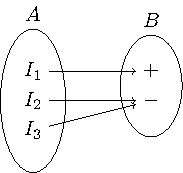
\includegraphics[scale=1.]{mapping}
  \caption{A classifier is a mapping between the group of instances and the group of categories or labels}
  \label{Fig:mapping}
\end{figure}
Some models produce a continuous output (estimation of and instance's class membership probability) to which different thresholds may be applied to predict class membership.

\end{frame}

\begin{frame}
  \frametitle{Confusion matrix (or contingency table)}
\label{sli:confusion}
  \begin{columns}
    \begin{column}{0.5\textwidth}
    
       
  \noindent
  \renewcommand\arraystretch{1.5}
  \setlength\tabcolsep{0pt}
  \begin{centering}
  \begin{tabular}{c >{\bfseries}r @{\hspace{0.7em}}c @{\hspace{0.4em}}c @{\hspace{0.7em}}l}
    \multirow{10}{*}{\rotatebox{90}{\parbox{3.1cm}{\bfseries\centering Hypothesized\\ class}}} & 
      & \multicolumn{2}{c}{\bfseries True class} & \\
    & & \bfseries p & \bfseries n  \\
    & Y & \MyBox{True}{Positives} & \MyBox{False}{Positives} \\[2.4em]
    & N & \MyBox{False}{Negatives} & \MyBox{True}{Negative} \\
    & total & P & N 
    \end{tabular}
\end{centering}
\end{column}
\begin{column}{0.5\textwidth}
\begin{tabular}{c}
  $\mathrm{FPR} = \frac{FP}{N}=1-\mathrm{TPR}$ \\ 
  $\mathrm{TPR} = \frac{TP}{P}=1-\mathrm{FPR}$\\
  $\mathrm{precision} = \frac{\mathrm{TP}}{\mathrm{TP}+\mathrm{FP}}$\\
  $\mathrm{recall\, (or\, sensitivity)} = \frac{\mathrm{tp}}{\mathrm{tp}+\mathrm{fn}}$\\
  $\mathrm{accuracy} = \frac{TP+TN}{P+N}$\\
  $\mathrm{F_{measure}}=\frac{2}{1/\mathrm{precision}+1/\mathrm{recall}}$
\end{tabular}
\end{column}
\end{columns}
sensitivity = recall = hit rate = TPR // specificity = selectivity = TNR
\end{frame}

\begin{frame}{ROC space}
  An ROC grph depicts relative tradeoffs between befeits (TP) and costs (FP).
  \begin{columns}
    \begin{column}{0.4\textwidth}
  \begin{figure}
  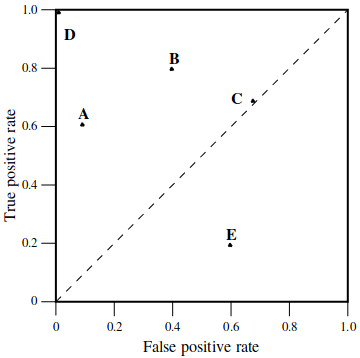
\includegraphics[width=0.8\linewidth]{ROC}
  \caption{Several examples of a discrete classifier\cite{fawcettIntroductionROCAnalysis2006}.}
\end{figure}
\end{column}
\begin{column}{0.6\textwidth}
  \begin{itemize}
    \item $(0,0)$ strategy of never issuing a positive classification
    \item $(1,1)$ unconditional issuing positive classifications
    \item $(0,1)$ perfect classification
    \item $(\approx 0, \approx 0)$ {\em Conservative} classifiers (few errors, but strong evidence for positives)
    \item $(\approx 1, \approx 1)$ {\em Liberal} classifiers (more positive with weak evidence)
  \end{itemize}
\end{column}
\end{columns}
\end{frame}

\begin{frame}{Some interesting regions}
  \begin{itemize}
    \item Random performance $y=x$
    \item To get away from the diagonal, the classifier should exploit some information in the data.
    \item Any classifier that generates a point in the lower right triangle can be {\em negated} to produce a dot in the upper left triangle.
    \item The question is: is a classifier slightly better than random signifficative or is it only better than random by chance? To answer this, we move into ROC curves.
  \end{itemize}

\end{frame}

\begin{frame}{ROC curves}
  \begin{enumerate}
    \item {\em Discrete classifiers} (decision trees or rule sets) only produce one point in the ROC space: a single confusion matrix. They can be transformed into a curve if we generate a score from the values obtained.
    \item {\em Probabilistic classifiers} produce an instance an strict probability or an uncalibrated score (Naive Bayes or neural networks). We can set up a threshold to produce a binary (discrete) classifier $\{\uvec{Y},\uvec{N}\}$.
  \end{enumerate}
\end{frame}

\begin{frame}{ROC curves}
 \begin{columns}
  \begin{column}{0.5\textwidth}
    \begin{figure}
    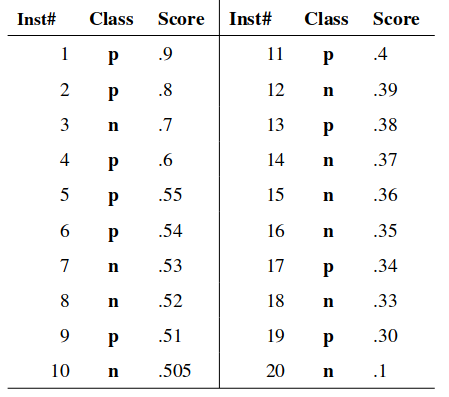
\includegraphics[width=0.8\linewidth]{tableROC}
    \end{figure}
  \end{column}
  \begin{column}{0.5\textwidth}
    \begin{figure}
    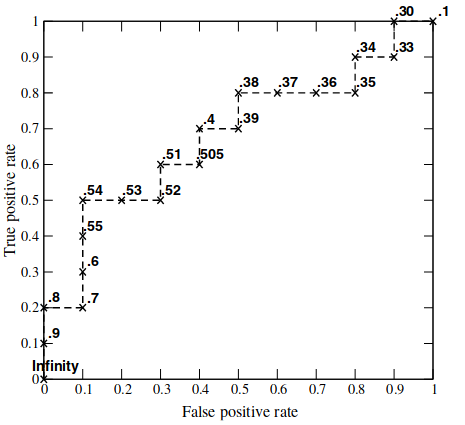
\includegraphics[width=0.8\linewidth]{ROCcurve}
    \end{figure}
  \end{column}
 \end{columns}
 The ROC curve created by thresholding a test set (adapted from \cite{fawcettIntroductionROCAnalysis2006}).
\end{frame}

\begin{frame}{Missclassification error and accuracy}
  Remember than in the binary classification case ($c=2$), and using the indicator loss function, the missclassification error can be written as:
  \[
    \mathrm{error} = \frac{\mathrm{FP}+\mathrm{FN}}{P+N}  
  \]
  and the accuracy can be calculated by measuring the fraction of correctly classified objects:
  \[
    \mathrm{accuracy} = 1 -   \mathrm{error} = \frac{\mathrm{TP}+\mathrm{TN}}{P+N}
  \]
  ROC graphs measure the ability of a classifier to produce good relative instance scores, able to discriminate between positive and negative instances.
\end{frame}

\begin{frame}{Relative vs absolute scores}
  \begin{figure}
    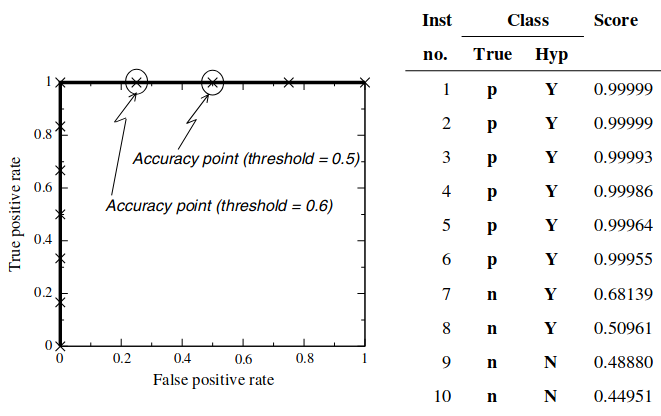
\includegraphics[width=0.7\textwidth]{ROCNaiveBayes}
    \caption{Accuracy vs ROC: score (not properly calibrated) and classification of 10 Naive Bayes instances, and the resulting ROC curves\cite{fawcettIntroductionROCAnalysis2006}.}
  \end{figure}
\end{frame}

\section{Precision-Recall curves}

\begin{frame}{Precision-Recall curves}
  The precision-recall curve shows the tradeoff between precision and recall for different threshold. A high area under the curve represents both high recall and high precision, where high precision relates to a low false positive rate, and high recall relates to a low false negative rate.  
  \\[10pt]
  As deduced from Slide \ref{sli:confusion}, ROC curves are insensitive to changes in class distribution: if the proportion of positive to negative instances changes in a test set, the ROC curves will not change! Accuracy, precision or $F$ score are sensitive to class skews.
\end{frame}

\begin{frame}{Precision-Recall curves}
  \begin{figure}
    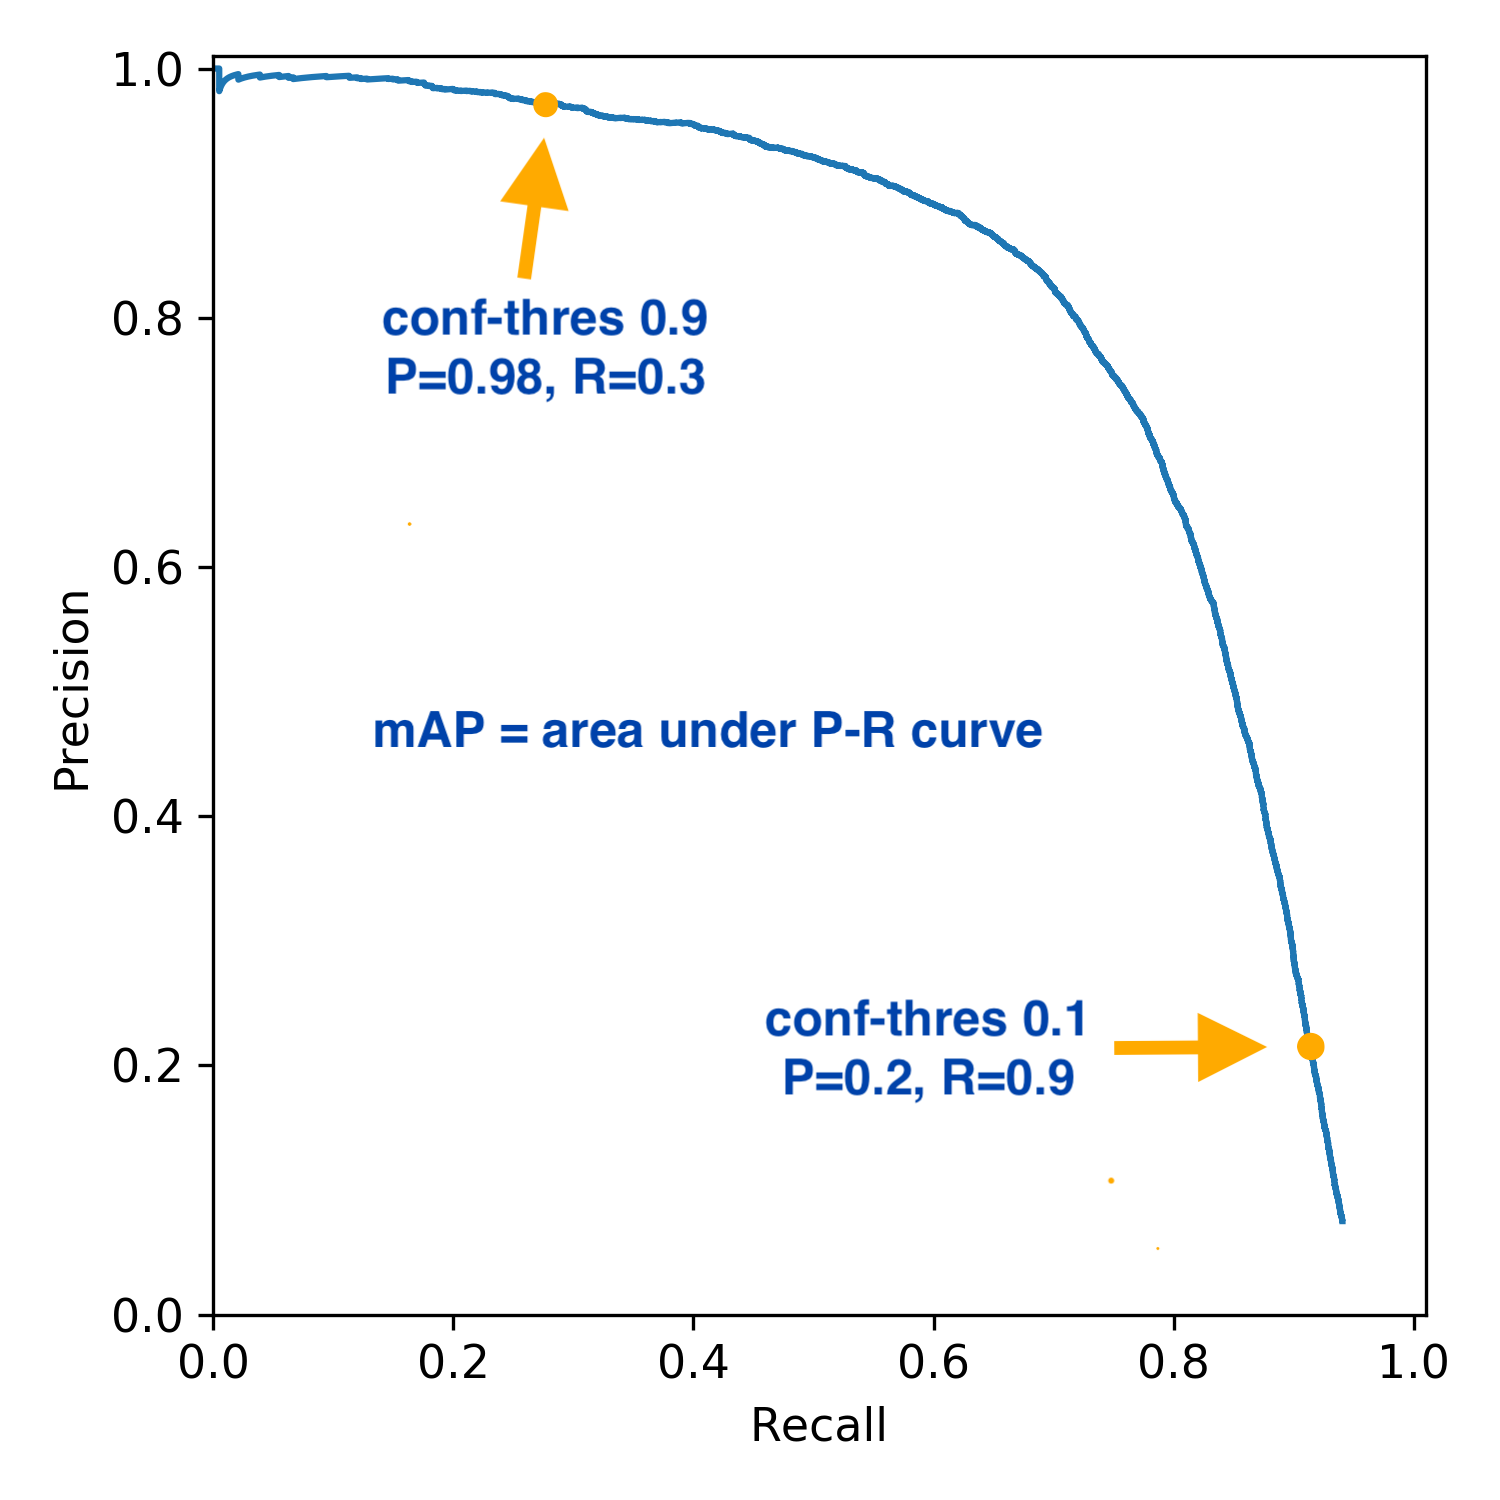
\includegraphics[width=0.5\textwidth]{PrecisionRecall}
    \caption{\href{https://github.com/ultralytics/yolov3/issues/898}{Example} of precision-recall curve.}
  \end{figure}
\end{frame}

\begin{frame}{Class skew}
  \begin{figure}
    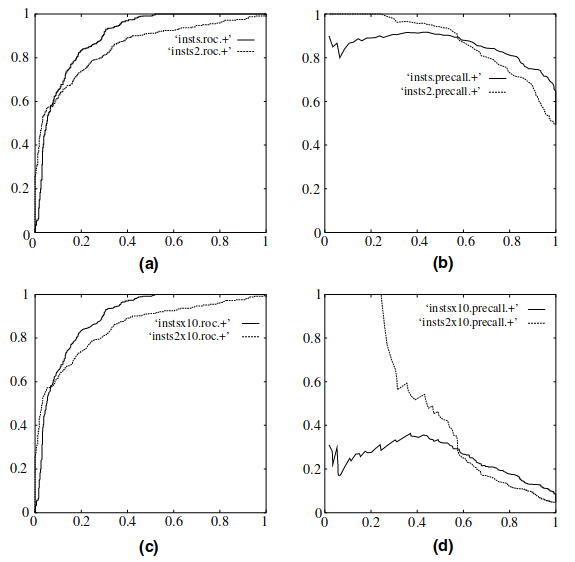
\includegraphics[width=0.5\textwidth]{PrecisionRecallROC}
    \caption{ROC and precision-recall curves under class skew. a-b) 1:1 rates; c-b) 1:10 rates; a-c) ROC curves; b-c) PR curves\cite{fawcettIntroductionROCAnalysis2006}.}
  \end{figure}
\end{frame}

\section{The convex ROC hull}

\begin{frame}{Convex hull}
  \begin{figure}
    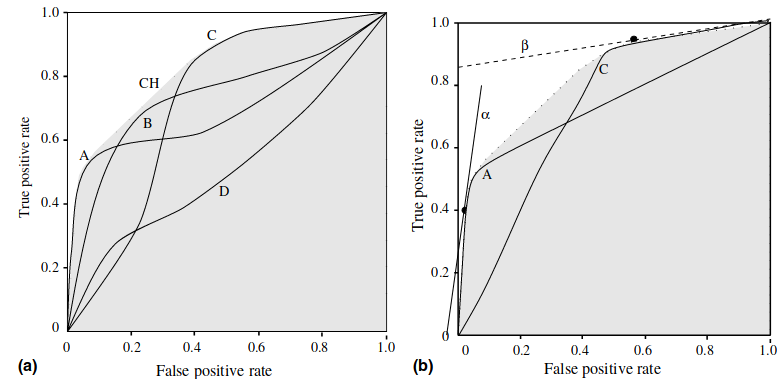
\includegraphics[width=0.6\textwidth]{ROCconvexhull}
    \caption{(a) Potentially optimal classifiers from ROC curves. Isoperformance line: $\frac{TP_2-TP_1}{FP_2-FP_1}=m$ for points with same expected cost. (b) Lines $\alpha$ and $\beta$ show the optimal classifier under different sets of conditions\cite{fawcettIntroductionROCAnalysis2006}.}
  \end{figure}
\end{frame}


\begin{frame}{Area under the curve (AUC)}
  The AUC of a classifier is equivalent to the probability that the classifier will rank a randonmly chosen positive instance higher than a randomly chosen negative instance (equivalent to Wilcoxon test of ranks)\cite{fawcettIntroductionROCAnalysis2006}.
  \begin{figure}
    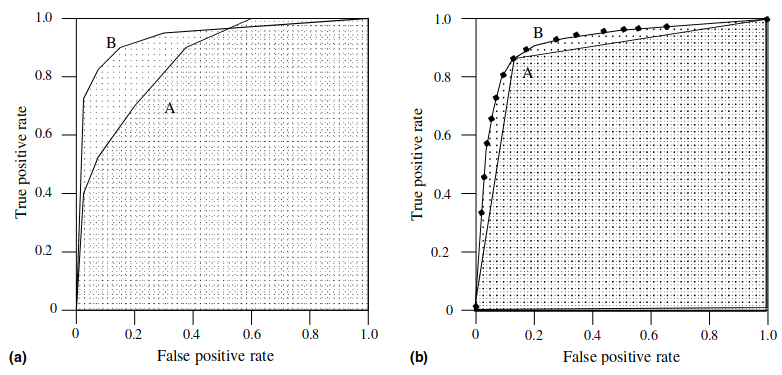
\includegraphics[width=0.7\textwidth]{AUC}
  \end{figure}
\end{frame}

\begin{frame}{A complete example\cite{swetsBetterDecisionsScience2000}}
  STEP 1: sample population of people whose eye pressure level and glaucoma status is known.
  \begin{figure}
    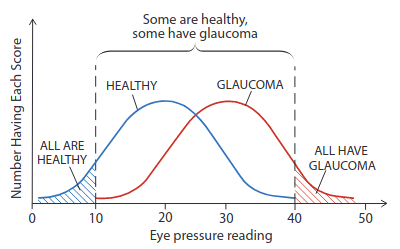
\includegraphics[width=0.7\textwidth]{ROCEx1}
    %\caption{ROC and precision-recall curves under class skew. a-b) 1:1 rates; c-b) 1:10 rates; a-c) ROC curves; b-c) PR curves\cite{fawcettIntroductionROCAnalysis2006}.}
  \end{figure}
\end{frame}

\begin{frame}{A complete example\cite{swetsBetterDecisionsScience2000}}
  STEP 2: determine the fraction of patients in the same population who would have properly diagnosed if a given threshold was applied
  \begin{figure}
    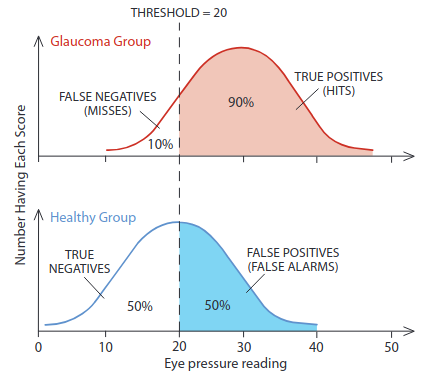
\includegraphics[width=0.5\textwidth]{ROCEx2}
    %\caption{ROC and precision-recall curves under class skew. a-b) 1:1 rates; c-b) 1:10 rates; a-c) ROC curves; b-c) PR curves\cite{fawcettIntroductionROCAnalysis2006}.}
  \end{figure}
\end{frame}

\begin{frame}{A complete example\cite{swetsBetterDecisionsScience2000}}
  STEP 3: build a ROC curve for the different threshold values
  \begin{figure}
    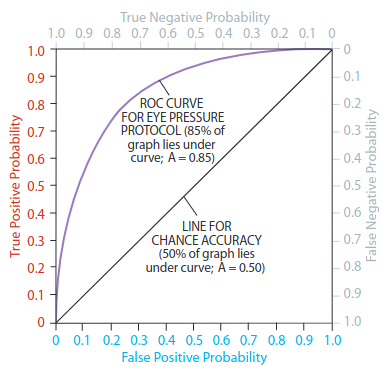
\includegraphics[width=0.5\textwidth]{ROCEx3}
    %\caption{ROC and precision-recall curves under class skew. a-b) 1:1 rates; c-b) 1:10 rates; a-c) ROC curves; b-c) PR curves\cite{fawcettIntroductionROCAnalysis2006}.}
  \end{figure}
\end{frame}

\begin{frame}{A complete example\cite{swetsBetterDecisionsScience2000}}
  STEP 4: select a threshold for yes/no diagnoses. Threshold chosen may often depend on subjective factors.
  \begin{figure}
    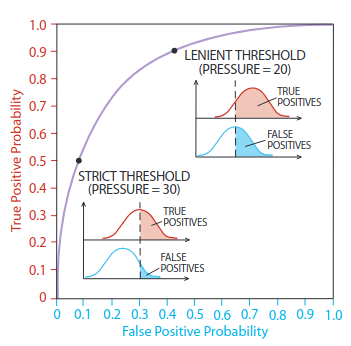
\includegraphics[width=0.5\textwidth]{ROCEx4}
    %\caption{ROC and precision-recall curves under class skew. a-b) 1:1 rates; c-b) 1:10 rates; a-c) ROC curves; b-c) PR curves\cite{fawcettIntroductionROCAnalysis2006}.}
  \end{figure}
\end{frame}

\begin{frame}{Practical implementation in python}
  Many examples of practical implementation of a ROC and precision recall curves in python are available. See, e.g., \href{https://machinelearningmastery.com/roc-curves-and-precision-recall-curves-for-classification-in-python/}{this example}.
\end{frame}
\section{Bibliography}
\bibliographystyle{unsrt}
\bibliography{DataSciencewithPython}
\end{document}